Peter Higgs naci\'o en 1929 en Newcastle, Inglaterra, por lo qu\'e
pas\'{o} su juventud parcialmente durante la Segunda Guerra Mundial,
circunstancias que complicaron un poco su formaci\'on escolar.
Despu\'es de la guerra, estudi\'o en Londres, primero matem\'aticas,
luego f\'isica. En 1954, con s\'olo 25 a\~nos termin\'o su
doctorado en el {\it King's College.}

Luego trabaj\'{o} temporalmente en la Universidad de Edimburgo,
en el {\it University College} y en el {\it Imperial College,} ambos
en Londres.
En 1960 regres\'{o} a Edimburgo -- ciudad que le encant\'o y donde
hab\'ia llegado por primera vez en 1949, como estudiante viajando
con {\it auto-stop} -- para ocupar un puesto de catedr\'{a}tico y
quedarse ah\'{\i} toda su vida.

En 1964, a los 35 a\~{n}os, escribi\'o sus dos art\'{\i}culos famosos
(y otro sobre el mismo tema en 1966) \cite{Higgs} que llamaron la
atenci\'{o}n y condujeron a invitaciones para presentar seminarios en
Princeton y Harvard en 1966. Ten\'{\i}a que tratar con audiencias cr\'iticas,
Sidney Coleman coment\'{o} m\'{a}s tarde que en Harvard ``quer\'ian
romper en pedazos al idiota que pensaba que pod\'ia evadir el
Teorema de Goldstone'' \cite{boson}. Result\'{o} que su concepto sigu\'io
de pie, pero a\'un sin aplicaci\'{o}n fenomenol\'{o}gica
(sus art\'iculos trataron con un modelo de juguete). Adem\'{a}s
se enter\'{o} por Yoichiro Nambu (el \'arbitro de uno de sus
art\'iculos) de un trabajo parecido \cite{EB}, publicado
15 d\'ias antes del primer art\'iculo de Higgs sobre el tema.
Los autores eran Fran\c{c}ois Englert y Robert Brout quienes
trabajaron en Bruselas, B\'elgica. Dos meses despu\'{e}s apareci\'{o}
otro art\'{\i}culo relacionado, escrito en Londres por
Gerald Guralnik, Carl Hagen y Tom Kibble \cite{GHK}, pero ellos
conocieron y citaron los trabajos anteriores de Englert, Brout y Higgs.



El mecanismo que estos tres art\'{\i}culos propusieron no era
totalmente nuevo: hab\'ia sido establecido en 1962/3 en el contexto de la
materia condensada por Philip Anderson \cite{Anderson}. \'El aplic\'o
conceptos de Julian Schwinger \cite{Schwinger} para la explicaci\'on
te\'orica de la masa de una part\'icula de norma a la teor\'ia de
superconductores. Englert, Brout y Higgs presentaron una
extensi\'on a modelos relativistas.

\begin{figure}[h]
	\centering
	\begin{subfigure}{0.3\textwidth}
	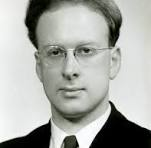
\includegraphics[scale=0.8]{images/higgs_joven.jpeg}
	\caption{}
	\end{subfigure}
	\begin{subfigure}{0.6\textwidth}
	\centering
	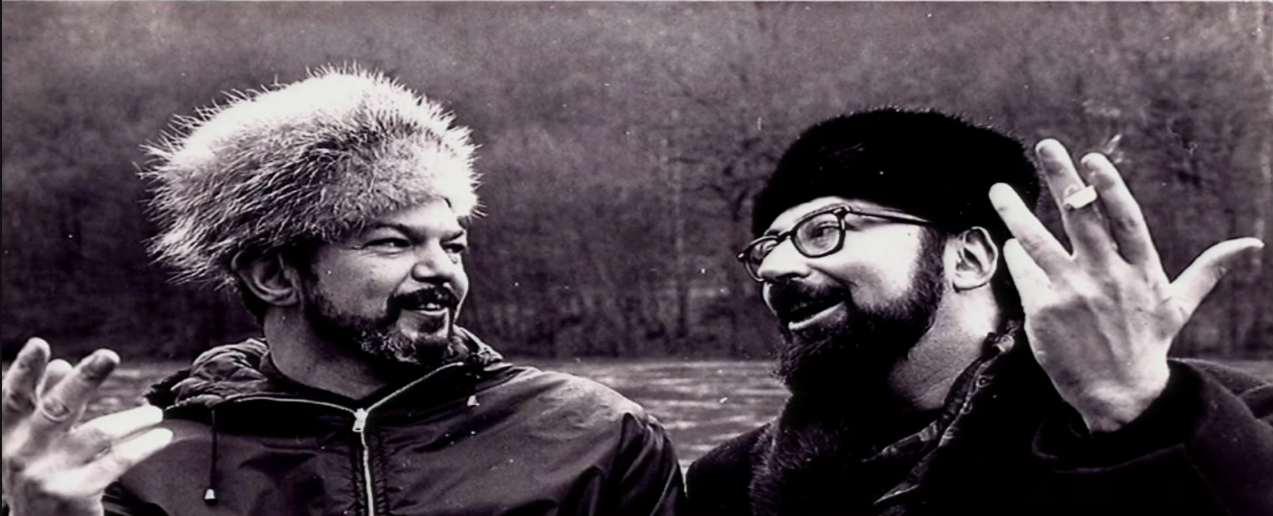
\includegraphics[scale=0.25]{images/brout_englert.png}
	\caption{}
	\end{subfigure}
	\caption{(a) Peter Higgs, quien public\'o dos art\'iculos breves sobre
        el ahora llamdo mecanismo de Higgs en 1964, y otro m\'as extenso
        en 1966. (b) Robert Brout
        (izquierda) y Fran\c{c}ois Englert (derecha). Brout invit\'o a
        Englert a trabajar en la Universidad de Cornell en 1959 por
        dos años como investigador asociado. Despu\'es
        Brout y Englert dejaron Cornell para trabajar en la
        Universidad de Bruselas, B\'elgica.}
	\end{figure}
\begin{figure}
\centering
\begin{subfigure}{0.31\textwidth}
	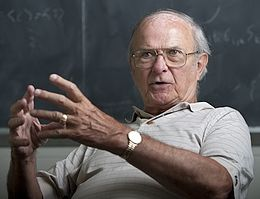
\includegraphics[scale=2]{images/hagen.jpg}
\end{subfigure}	
\begin{subfigure}{0.31\textwidth}
	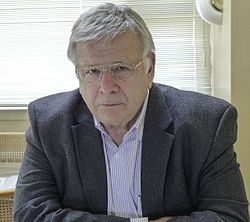
\includegraphics[scale=0.5]{images/guralnik.jpg}
\end{subfigure}	
\begin{subfigure}{0.31\textwidth}
	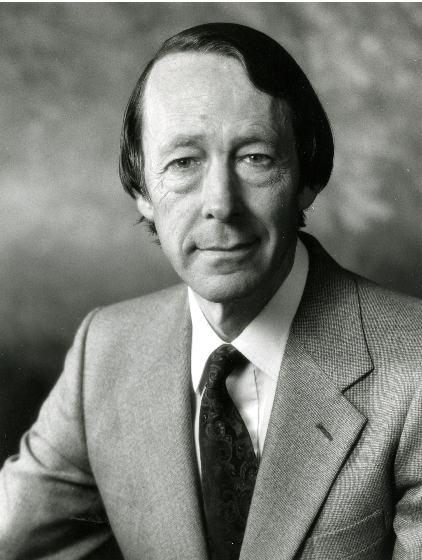
\includegraphics[scale=0.25]{images/kibble.png}
\end{subfigure}	

	\caption{Los otros descubridores del mecanismo de Higgs.
        De izquierda a derecha, Carl Hagen, Gerald Guralnik y Tom Kibble.} 
\end{figure}

\begin{figure}[h]
\centering
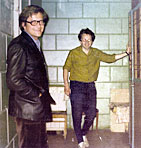
\includegraphics[scale=1]{images/polyakov_migdal.jpg}	
\caption{Cuando a\'un eran {\it teenagers}, Alexander
Migdal (izquierda) y Alexander Polyakov (derecha) descubrieron
independiente del occidente el principio del mecanismo de Higgs.}
\end{figure}


	\begin{figure}
			\begin{subfigure}{0.5\textwidth}
	\centering	
		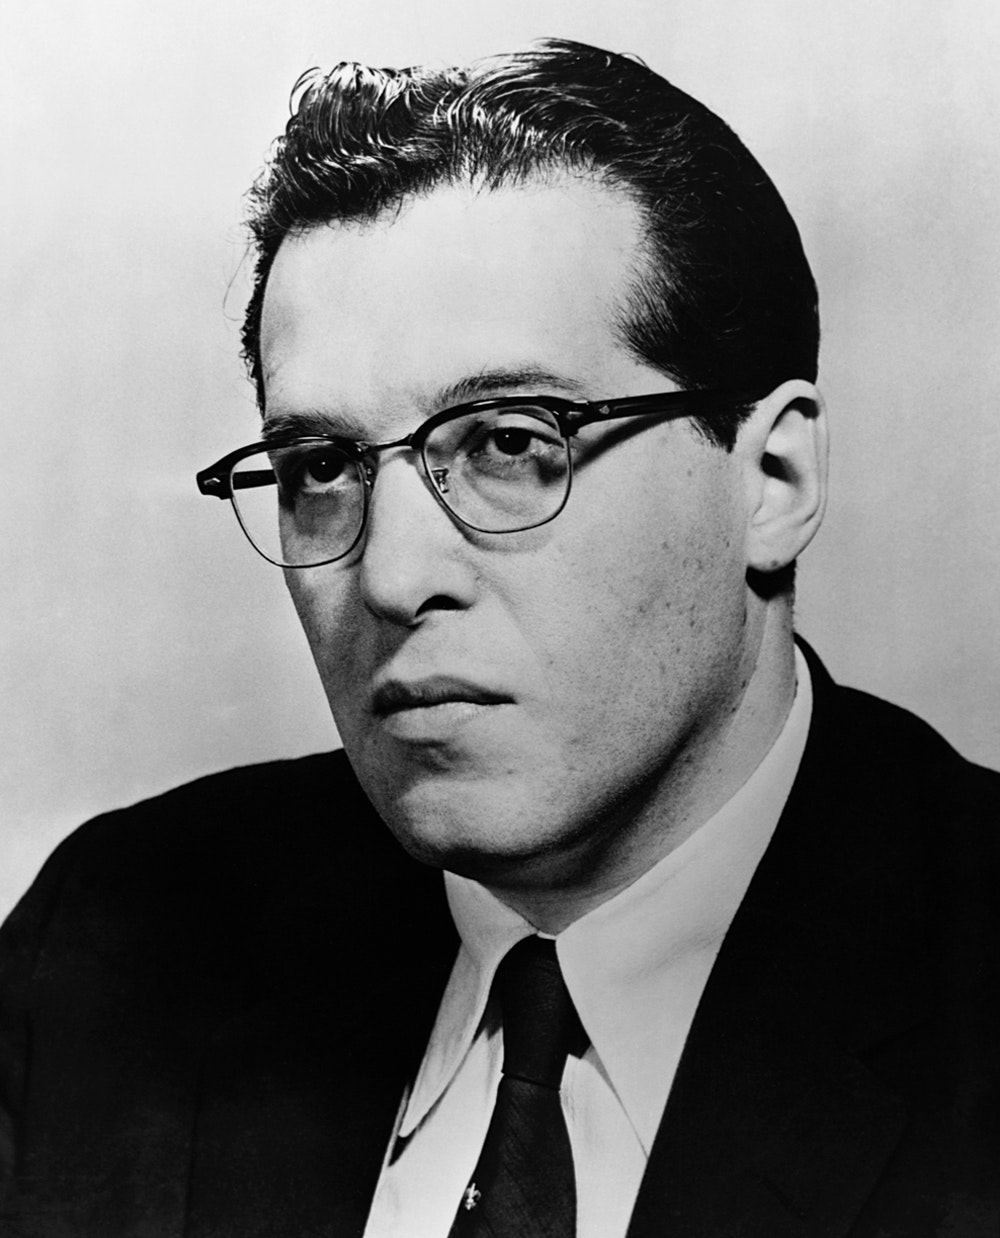
\includegraphics[scale=0.15]{images/schwinger.jpg}
	\end{subfigure}
	\begin{subfigure}{0.5\textwidth}
	\centering	
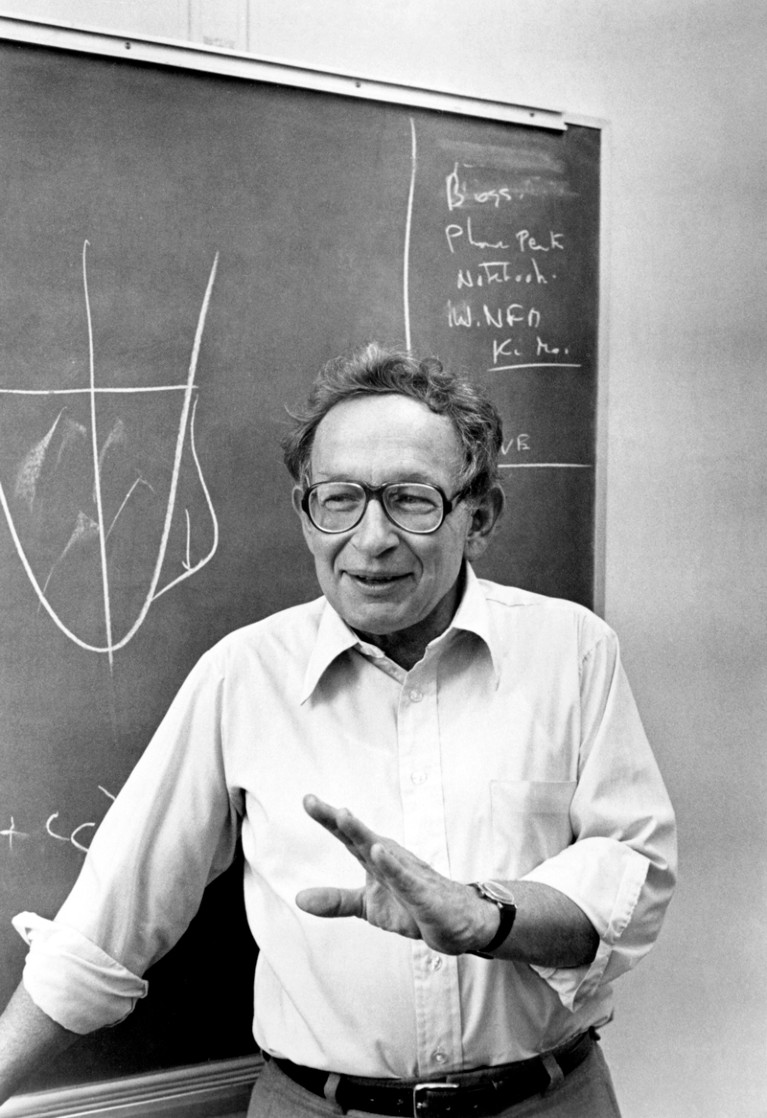
\includegraphics[trim = {1cm 1cm 4cm 12cm},clip,scale=0.25]{images/anderson.jpg}
		\end{subfigure}
\caption{Izquierda: Julian Schwinger, podemos trazar el descubrimiento
del mecanismo de Higgs a su trabajo pionero sobre c\'omo una simetr\'ia de norma no siempre implicaba un bos\'on de norma no masivo. Derecha: Philip Anderson descubri\'o el mecanismo que da
masa a los bosones de norma en el contexto de la superconductividad.}
	\end{figure}

\begin{figure}[h]
\centering
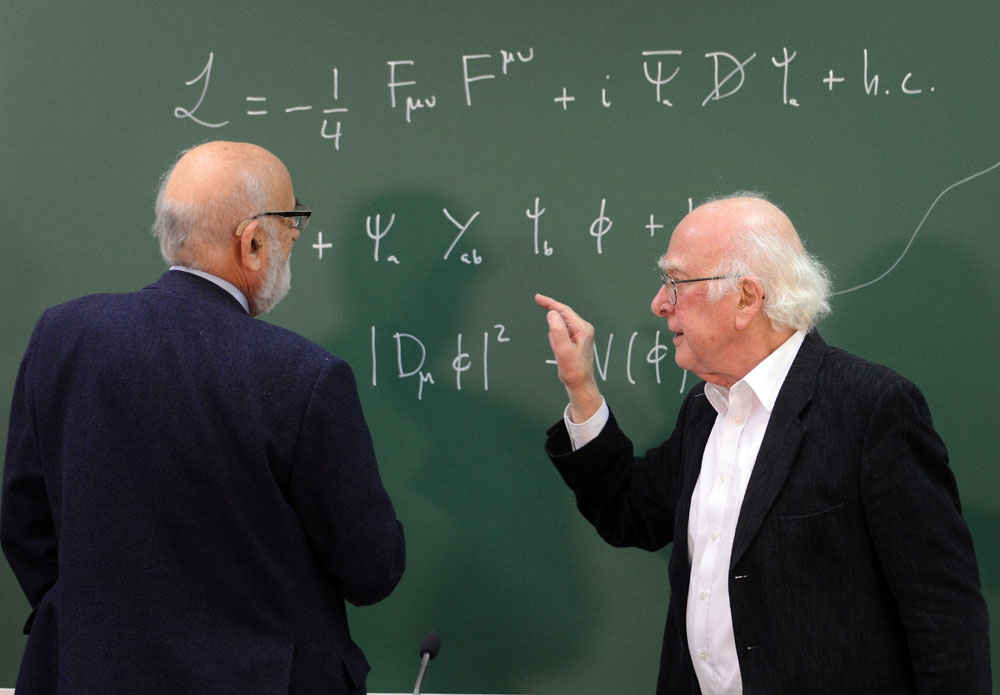
\includegraphics[scale=0.3]{images/higgs_englert_pizarra.jpeg}
\caption{Peter Higgs y Fran\c{c}ois Englert discutiendo el lagrangiano
que involucra al ahora llamado campo de Higgs, $\phi$.
?`Qu\'e creen que Higgs le dice a Englert? Tal vez le indique que
en la segunda l\'inea falta una barra en el campo fermi\'onico
$\bar \psi_a$.}
\end{figure}


Totalmente independientemente, en Mosc\'{u} en 1965, dos chicos de 19
a\~nos, ambos de nombre Alexander (o Sasha), con apellidos Migdal y
Polyakov, discutieron en gran detalle qu\'e significa el rompimiento
de una simetr\'ia \cite{Nobel13}. Ellos escribieron otro art\'iculo
parecido que fue publicado en 1966 \cite{MigPol}. Hace unos
a\~{n}os que Migdal visit\'o M\'exico y
% para un evento organizado por Alexander Turbiner, donde
relat\'o sobre las dificultades que ten\'{\i}an para publicar
este art\'iculo, ya qu\'e la comunidad de f\'{\i}sicos establecidos
en la Uni\'on Sovi\'etica -- bajo el liderazgo de Lev Landau -- rechaz\'o
la teor\'{\i}a cu\'antica de campos, que todav\'{\i}a era muy
controversial tambi\'en en el mundo occidental.\footnote{En Alemania
Werner Heisenberg era oponente influyente contra la teor\'ia cu\'antica
de campos; su preferencia era el formalismo de la matriz S.}
Finalmente, este art\'iculo
fue publicado algo tarde, pero despu\'es ambos Sashas se hicieron
famosos por otros trabajos --- en especial, Polyakov es conocido por
descubrir excitaciones topol\'ogicas que llamamos ahora instantones.

La explicaci\'on de c\'omo  las part\'iculas de norma -- y ciertas part\'iculas
acopladas -- pueden tener masa fue pronto conocida como el {\em mecanismo
de Higgs},\footnote{Consultar la literatura original no conduce a
  una explicaci\'on muy clara cu\'al es realmente la raz\'on por la que la
  terminolog\'ia excluye a Brout y Englert.}
  el tema de la Secci\'on 2 de este art\'iculo.
Su aplicaci\'on a la fenomenolog\'ia de part\'iculas elementales 
emergi\'o en 1967/8 por parte de Steven Weinberg \cite{Weinberg} y
Abdus Salam \cite{Salam}.
Ellos integraron este mecanismo al modelo de la interacci\'on
electrod\'ebil que Sheldon Glashow hab\'ia propuesto en 1961
\cite{Glashow} durante su estancia en Copenhague.
De hecho, Glashow estuvo presente en el seminario de Higgs en Harvard,
y reconoci\'o que era {\it ``a nice model''} \cite{boson}, pero no se le
occuri\'o la idea de que este mecanismo podr\'ia ser el remedio
para salvar a su modelo, que \'el ya hab\'ia abandonado.

Sin embargo, esta teor\'ia -- ahora conocida como el sector
electrod\'ebil del Modelo Est\'andar -- a\'un no era generalmente
aceptada ya que era considerada ``no renormalizable''.
En las teor\'ias cu\'anticas de campos casi siempre aparecen divergencias
a altas energ\'ias, as\'i que requieren una ``regularizaci\'on'',
una manipulaci\'on matem\'atica que convierte las divergencias
en un valores finitos. Se dice que una teor\'ia es {\em renormalizable}
si, al final del c\'alculo, se puede remover la regularizaci\'on
totalmente y llegar a predicciones finitas para las observables
(esta definici\'on es ligeramente simplista).

La comunidad f\'isica cambi\'o su punto de vista en 1971/2, gracias
al trabajo de Gerard 't Hooft, un brillante estudiante de doctorado
en Utrecht, Holanda, quien present\'o evidencia a favor de la
renormalizibilidad de dicho modelo (parcialmente junto a
su asesor, Martinus Veltman). Estos trabajos \cite{tHooft} fueron
una sensaci\'on que causaron un cambio de paradigma en aquella \'epoca.

\begin{figure}
\begin{subfigure}{0.5\textwidth}
	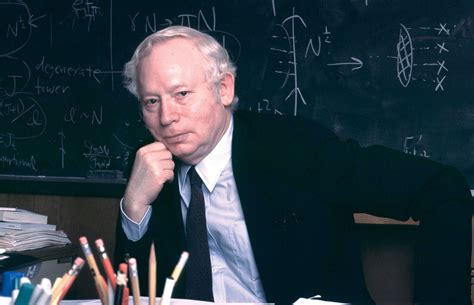
\includegraphics[scale=0.5]{images/weinberg.jpeg}
\end{subfigure}	
\begin{subfigure}{0.5\textwidth}
	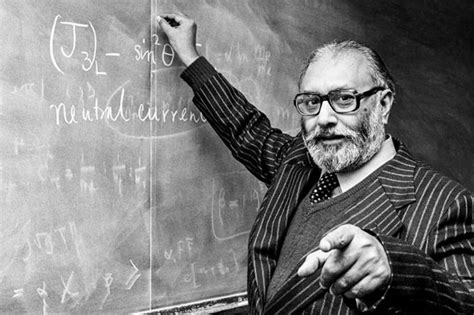
\includegraphics[scale=0.5]{images/salam.jpeg}
\end{subfigure}	
\caption{Steven Weinberg (izquierda) y Abdus Salam (derecha)
independientemente integraron el mecanismo de Higgs al sector
electrod\'ebil del Modelo Est\'andar.}
%Ambos compartieron el Premio
%Nobel de f\'isica en 1979 junto a Sheldon Glashow.}
\end{figure}

\begin{figure}
\centering
\begin{subfigure}{0.5\textwidth}
\centering
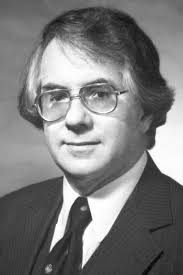
\includegraphics[scale=0.45]{images/glashow.jpeg}
\end{subfigure}\begin{subfigure}{0.5\textwidth}
\centering
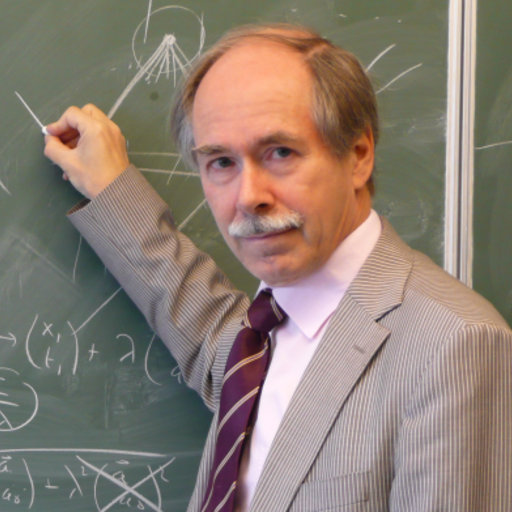
\includegraphics[scale=0.25]{images/thooft.jpg}
\end{subfigure}
\caption{Izquierda: Sheldon Glashow, creador de la versi\'on orignal
de la teor\'ia electrod\'ebil. Derecha: Gerard 't Hooft, famoso por
%fue galardonado
%con el Premio Nobel de f\'isca en 1999 debido a
su trabajo sobre la renormalizaci\'on del Modelo Est\'andar,
entre otras cosas.}
\end{figure}

La clave para este hito fue un nuevo m\'etodo, la {\em regularizaci\'on
dimensional} que est\'a entre los logros principales de la f\'isica en
Am\'erica Latina: fue propuesta primero por dos argentinos, Carlos Bollini
y Juan Jos\'e Giambiagi en 1971, aunque la publicaci\'on \cite{BolGiam}
se demor\'o hasta 1972. Ellos trabajaron en La Plata, en
circunstancias dif\'iciles durante la dictadura militar \cite{DimReg}.

Agregamos que hoy en d\'ia se da menos importancia a la pregunta
si el Modelo Est\'andar es renormalizable o no: la tendencia es que se
considera como teor\'ia efectiva, y su validez en un gran rango
energ\'etico -- que no tiene que extenderse hacia infinito --
es suficiente.

Poco despu\'es, en 1973, el Modelo Est\'andar de las part\'iculas
elementales fue completamente establecido, con un sector
electrod\'ebil \cite{Weinberg,Salam} y otro de la interacci\'on
fuerte \cite{QCD}. El mecanismo de Higgs es indispensable para
proporcionar masas a gran parte de las part\'iculas elementales.
Esto fue una revoluci\'on en la f\'isica de altas energ\'ias como no la
hemos visto m\'as en el medio siglo que sigui\'o, ya que despu\'es el
progreso fue relativamente lento.




En el siglo XXI es popular especular sobre f\'isica m\'as all\'a
del Modelo Est\'andar. Sin embargo, por ahora ninguna de estas propuestas
tiene apoyo s\'olido de datos experimentales. Por otro lado, los
experimentos han confirmado las predicciones del Modelo Est\'andar una
y otra vez: muchas veces salen al aire en las noticias que el
Modelo Est\'andar ha sido ``refutado''
por nuevos resultados, pero al final del an\'alisis, y la repetici\'on
de los experimentos, siempre sus predicciones han
triunfado.\footnote{Como ejemplo reciente, en la segunda parte de la
  d\'ecada pasada, se difundieron noticias de una tensi\'on entre el Modelo
  Est\'andar y experimentos con el decaimiento de mesones pesados
  conocidos como ``mesones B''. Al final, esta discrepacia no se
  substanci\'o. La \'ultima moda es el momento magn\'etico del
  mu\'on, donde el valor experimental parece un poquito diferente
  del c\'alculo basado en el Modelo Est\'andar. Si esto es verdad --
  cosa que no es nada segura -- la predicci\'on se equivoca al
  nivel relativo de $10^{-10}$: si lo comparamos con la distancia
  entre M\'exico y Europa central (Suiza por ejemplo), unos
  10,000\,km, esto corresponde a un posible error de la magntitud
  de mil\'imetros. Pero c\'alculos con simulaciones num\'ericas
  en la ret\'icula conducen a resultados m\'as cercanos al valor
  experimental, tendencia que indica que incluso esta discrepancia
  m\'inima podr\'ia desaparecer con un an\'alisis m\'as preciso,
  igual que todas las supuestas discrepancias anteriores.}
  
El Modelo Est\'andar es algo incompleto para describir al
universo (faltan por ejemplo la gravitaci\'on, materia oscura y
energ\'ia oscura), pero a\'un as\'i: se trata de nada menos que la
teor\'ia m\'as precisa y -- en este sentido -- m\'as exitosa en
la historia de la ciencia.\\
 
Higgs ya no particip\'o en este desarollo r\'apido. \'El ya era
tan famoso que pod\'ia permitirse casi no publicar m\'as resultados
de investigaci\'on a partir de la edad de 40 a\~{n}os.
(En M\'exico esto ser\'ia un problema serio con el SNII etc.)
 
Fue conocido como una persona tranquila y modesta, casi t\'imida,
que no busc\'o la atenci\'on medi\'atica o ponerse en el centro de
atenci\'on en eventos. Con su mentalidad de abstenerse del
{\it show,} se puede caracterizar como el contrario a Feynman.
Esta caracterizaci\'on corresponde a la impresi\'on de uno de los
autores (WB) qui\'en particip\'o en un congreso en Edimburgo 1997.
Higgs -- quien era em\'erito desde 1996 -- apareci\'o en el banquete,
pero muy discreto, simplemente para sentarse en una mesa sin
ning\'un espect\'aculo.

Esto no significa que Higgs no ten\'ia convicciones: fue
temporalmente activista por el desarmamento nuclear y
por el movimiento ambiental como miembro de {\it Greenpeace.}\\

Una vez que el Modelo Est\'andar hab\'ia sido establecido, su exploraci\'on
progres\'o con trabajo intenso en m\'ultiples pa\'ises.
En el a\~no 2000, todas sus part\'iculas ya eran experimentalmente
encontradas, menos una: la famosa ``part\'icula de Higgs'', involucrada
en este mecanismo, como vamos a describir en la Secci\'on 2.

Otra vez, la nomenclatura es tal vez un poco injusta con Englert y
Brout, pero as\'i es la convenci\'on de la comunidad.
Higgs no invent\'o este t\'ermino (esto lo hizo primero  Ben Lee
\cite{boson}), pero tambi\'en le era inc\'omodo el
apodo absurdo ``part\'icula de dios'' que no tiene ni el menor sentido.
Este t\'ermino fue propuesto por la editorial de un libro de divulgaci\'on
\cite{Lederman},
obviamente con un objetivo comercial, pero plenamente irresponsable.
Este t\'ermino se hizo popular y condujo a confusi\'on sin fin,
por ejemplo, la iglesia cat\'olica de Espa\~na crey\'o que el trabajo del
CERN tuviera algo que ver con teolog\'ia \cite{Guardian}. !`Tenemos que
tener cuidado con los t\'erminos que se usamos!

En el siglo XXI fuimos testigos de una carrera emocionante en la
b\'usqueda de la part\'icula de Higgs. En su fase final, era una
compentencia entre el Fermilab (cerca de Chicago) y el CERN
(cerca de Ginebra, sobre la frontera entre Suiza y Francia).
Despu\'es de primeras indicaciones en 2011, en 2012 las
colaboraciones ATLAS y CMS, ambos trabajando de manera independiente
en el Gran Colisionador de Hadrones (LHC) en el CERN, presentaron
evidencia indirecta pero clara de la observaci\'on de la
part\'icula de Higgs, que era tanto buscada \cite{ATLASCMS}.

	
\begin{figure}

\begin{subfigure}{0.5\textwidth}
	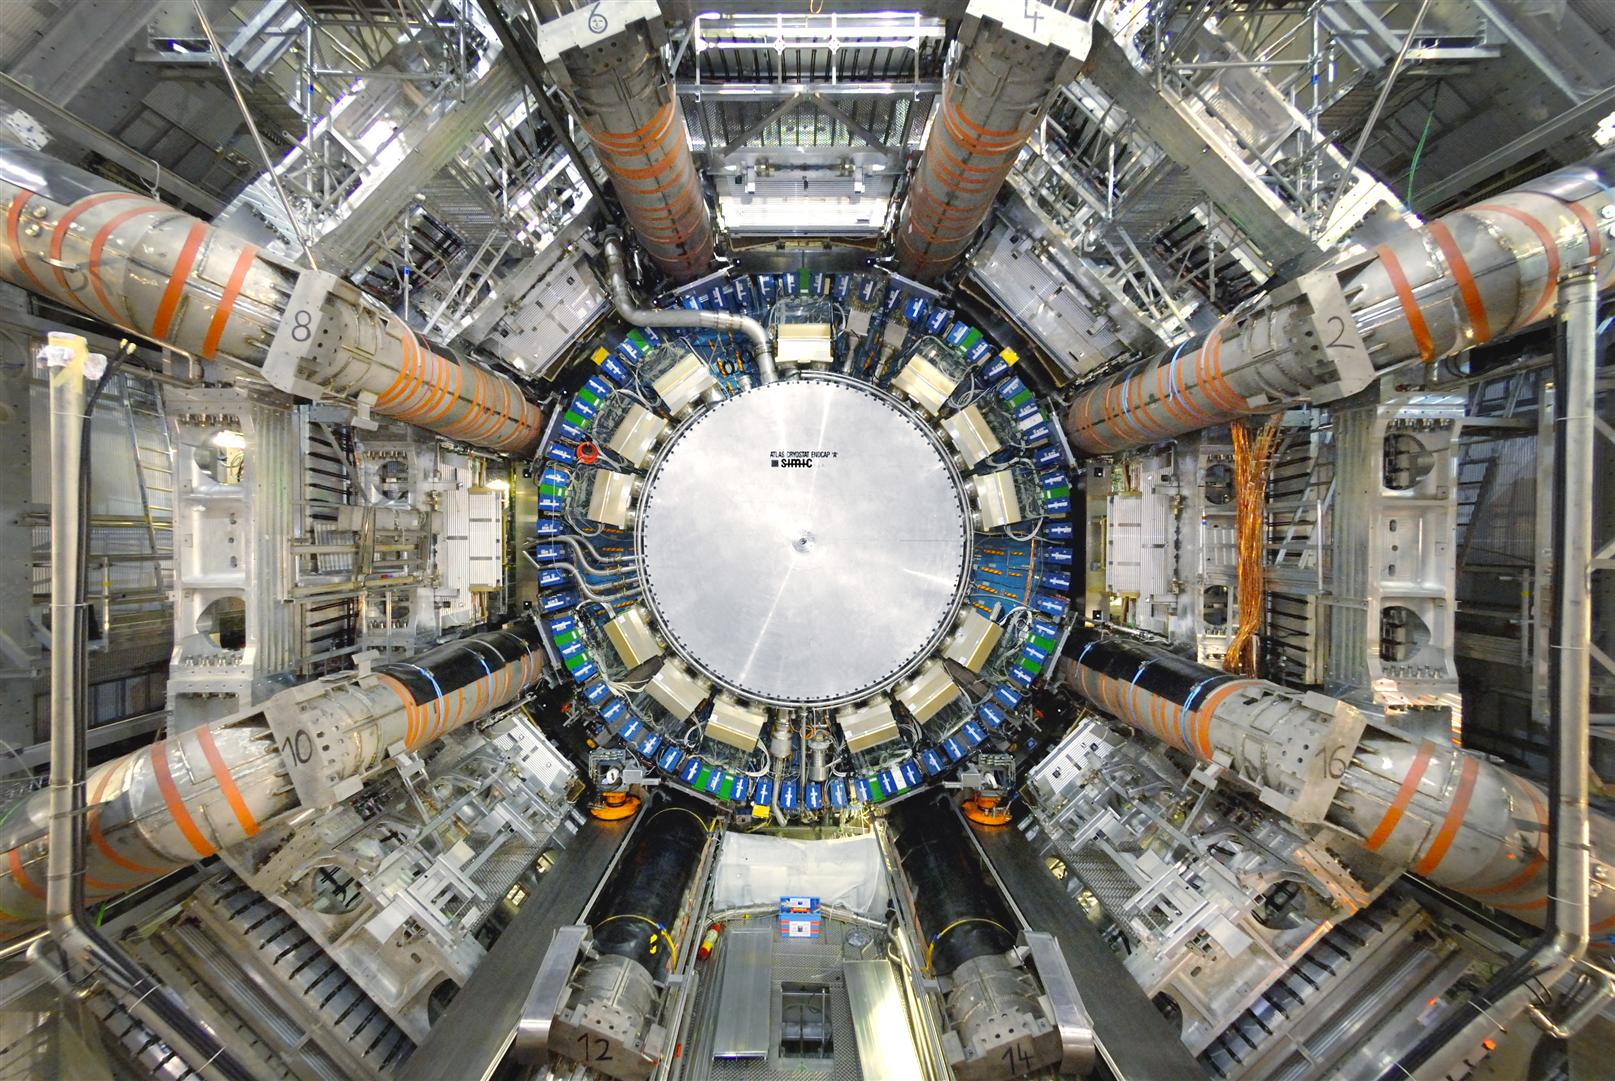
\includegraphics[scale=0.27]{images/atlas.jpg}
\end{subfigure}	
\begin{subfigure}{0.5\textwidth}
	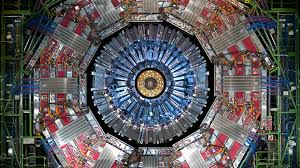
\includegraphics[scale=0.9]{images/cms.jpeg}
\end{subfigure}	
\caption{Detectores de la Colaboraci\'on ATLAS (izquierda) y CMS
(derecha) en el CERN que confirmaron las existencia del bos\'on
de Higgs del Modelo Est\'andar.
Ambos son detectores multiprop\'osito usados para
analizar colisiones entre part\'iculas de muy alta energ\'ia.}
\end{figure}


Con esto todo el conjunto de part\'iculas del Modelo Estandar
fue observado. As\'i se confirm\'o que el mecanismo de Higgs
est\'a realizado en la naturaleza, 48 a\~nos despu\'es de su
propuesta te\'orica. Esto se demor\'o casi el doble del tiempo
que la observaci\'on del neutrino (predicho por Wolfgang Pauli en 1930, y
detectado por Clyde Cowan, Frederick Reines y colaboradores en
1956),\footnote{Ref.\ \cite{neutrinos} revisa la historia y las
propiedades de los neutrinos, de una perspectiva semi-divulgativa.}
vemos que a veces vale la pena tener paciencia.

En particular, vali\'o la pena para Englert y Higgs, quienes recibieron
el Premio Nobel en 2013 por su predicci\'on correcta \cite{Nobel13};
tristemente, Brout hab\'ia muerto poco antes, en 2011.
En abril del 2024 nos lleg\'o la noticia del fallecimiento de Higgs,
a los 94 a\~nos, despu\'es de una breve enfermedad.

\begin{figure}
\centering
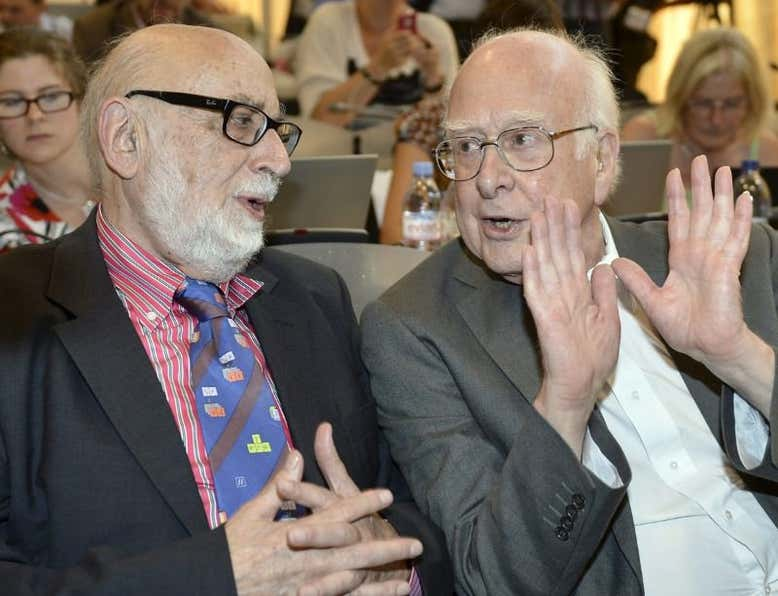
\includegraphics[scale=.3]{images/higgs_englert2.jpeg}
\caption{El 4 de julio de 2012 el CERN hizo p\'ublico el
descubrimiento del bos\'on de Higgs. Peter Higgs conmovido hasta
las l\'agrimas en la ceremonia dijo: ``Felicitaciones a todos los
involucrados en este descubrimento. Para m\'i es algo verdaderamente
incre\'ible que haya vivido para verlo''. La Real Academia Sueca de
las Ciencias otorg\'o el premio Nobel de F\'isica en 2013 a Fran\c{c}ois
Englert (izquierda) y a Peter Higgs (derecha) por ``el descubrimiento
te\'orico de un mecanismo que contribuye a nuestra comprensi\'on del
origen de la masa de las part\'iculas subat\'omicas $\dots$''
\cite{YouTube}.}
\end{figure}